\documentclass[11pt]{amsart}
\usepackage{geometry}                
\geometry{letterpaper}                   
\usepackage{graphicx,mathrsfs,epstopdf}
\usepackage{amsmath,amsfonts,amssymb,amsthm}
\usepackage[colorlinks,citecolor=blue,urlcolor=blue]{hyperref}
\usepackage{tikz}
\usetikzlibrary{positioning}
\DeclareGraphicsRule{.tif}{png}{.png}{`convert #1 `dirname #1`/`basename #1 .tif`.png}

%%%%%%%%%%%%%%%%%%%%%%%%%%%%%%%%%%
%theorems etc.
\newtheorem{thm}{Theorem}[section]
\newtheorem{lem}[thm]{Lemma}
\newtheorem{prop}[thm]{Proposition}
\newtheorem{cor}[thm]{Corollary}

\theoremstyle{definition}
\newtheorem{defn}[thm]{Definition}
\newtheorem{const}[thm]{Construction}
\newtheorem{conj}[thm]{Conjecture}
\newtheorem{exmp}[thm]{Example}
\newtheorem{assp}[thm]{Assumption}

\theoremstyle{remark}
\newtheorem{rem}[thm]{Remark}
\newtheorem{note}{Note}
\newtheorem{ques}{Question}

%operators

\DeclareMathOperator{\cent}{Cent} 
\DeclareMathOperator{\rk}{rk} \DeclareMathOperator{\cl}{cl}
\DeclareMathOperator{\Hom}{Hom} \DeclareMathOperator{\En}{End}
\DeclareMathOperator{\Exc}{Exc} \DeclareMathOperator{\Ker}{Ker}
\DeclareMathOperator{\Proj}{Proj}
\DeclareMathOperator{\Diff}{Diff}
\DeclareMathOperator{\Sing}{Sing}
\DeclareMathOperator{\Supp}{Supp}
\DeclareMathOperator{\Sec}{Sec}


%other commands

\newcommand{\QED}{\ifhmode\unskip\nobreak\fi\quad {\rm Q.E.D.}} % QED
\newcommand\recip[1]{\frac{1}{#1}}
\newcommand\fr[1]{\lfloor{#1}\rfloor}
\newcommand\frup[1]{\lceil{#1}\rceil}
\newcommand\Span[1]{\langle{#1}\rangle}
\newcommand\Ga{\Gamma}
\newcommand\map{\dasharrow}
\newcommand\iso{\cong}
\newcommand\la{\lambda}
\newcommand{\f}{\varphi}
\newcommand{\cA}{\mathcal{A}}
\newcommand{\C}{\mathbb{C}}
\newcommand{\cD}{\mathcal{D}}
\newcommand{\cE}{\mathcal{E}}
\newcommand{\cF}{\mathcal{F}}
\newcommand{\cG}{\mathcal{G}}
\newcommand{\cH}{\mathcal{H}}
\newcommand{\cI}{\mathcal{I}}
\newcommand{\cK}{\mathcal{K}}
\newcommand{\cL}{\mathcal{L}}
\newcommand{\cM}{\mathcal{M}}
\newcommand{\N}{\mathbb{N}}
\newcommand{\A}{\mathbb{A}}
\newcommand{\cO}{\mathcal{O}}
\renewcommand{\P}{\mathbb{P}}
\newcommand{\Q}{\mathbb{Q}}
\newcommand{\R}{\mathbb{R}}
\newcommand{\cS}{\mathcal{S}}
\newcommand{\T}{\mathbb{T}}
\newcommand{\Z}{\mathbb{Z}}
\newcommand{\cW}{\mathcal{W}}
\newcommand\Segre[1]{\Sigma_{#1}}
\newcommand\lag{\langle}
\newcommand\rag{\rangle}
\newcommand{\RLCT}{{\rm RLCT}}
\newcommand{\ind}{{\rm ind}}
\newcommand{\rank}{{\rm rank}}
\newcommand{\indep}{{\;\bot\!\!\!\!\!\!\bot\;}}
\newcommand{\indic}{{1\!\!1}}
\newcommand{\nmapsto}{{\;\mapsto\!\!\!\!\!\!\!\slash\;}}
\newcommand{\lr}{\leftrightarrow}
\newcommand{\pa}{{\rm pa}}
\renewcommand{\sp}{{\rm sp}}
\renewcommand{\ne}{{\rm ne}}
\newcommand{\an}{{\rm an}}
\newcommand{\de}{{\rm de}}
\newcommand{\bs}{\boldsymbol}

%%%%%%%%%%%%%%%%%%%%%%%%%%%%%%%%%%%
\def\proofname{\indent {\sl Proof.}}



\title{Gaussian graphical models with Macaulay2}
\author{}
\address{}
\curraddr{}
\email{}
\thanks{}

\date{\today}                                            % Activate to display a given date or no date

\begin{document}
\maketitle
\begin{abstract}
Very brief introduction to mixed graphs and some of my early ideas
\end{abstract}


\section{Gaussian models of mixed graphs}

Following \cite{sullivant2008tsg} we consider mixed graphs, that is graphs with undirected $i-j$, directed $i\to j$ and bidirected edges $\lr$ but with no multiple edges between any two vertices. We assume that there is a partition of vertices $U\cup W=V(G)$, such that if $i-j$ in $G$ then $i,j\in U$, if $i\lr j$ in $G$ then $i,j\in W$ and there is no directed edge $i\to j$ in $G$ such that $i\in W$ and $j\in U$. We also assume that the subgraph on directed edges is acyclic. With all these assumptions on mixed graphs, we can order vertices in such a way that all vertices in $U$ come before vertices in $W$, and whenever $i\to j$ we have $i<j$. Note that we allow a pair of vertices to be connected by both a directed edge $i\to j$ and bidirected edge $i\lr j$ or undirected edge $i-j$. With this setup, undirected graphs, DAGs, ancestral graphs \cite{RSancestral2002} and chain graphs \cite{andersson2001} occur as special cases.

For any mixed graph $G=(V,E)$ we define the associated Gaussian model $M(G)$ as the subset of all positive definite, symmetric matrices in $\R^{V\times V}$ of the form

 Denote by $\R^{V\times V}$ the set of matrices with rows and columns indexed by the nodes of $G$, where vertices in $V$ are ordered as described in the paragraph above. Let $G=(V,E)$ be a mixed graph as defined above and let $\bs X=(X_i)_{i\in V}$ be a Gaussian random vector with zero mean and covariance $\Sigma\in \cS^V_+$, where $\cS^V_+$ is the set of symmetric positive definite matrices in $\R^{V\times V}$ of the form
 \begin{equation}\label{eq:parametrization}
\Sigma\quad=\quad (I-\Lambda)^{-T}\left[\begin{array}{cc}
K^{-1} & \bs 0\\
\bs 0 & \Psi
\end{array}
\right](I-\Lambda)^{-1},
\end{equation}
where 
\begin{itemize}
\item[(i)] $\Lambda=[\lambda_{ij}]\in \R^{V\times V}$ is such that $\lambda_{ij}\neq 0$ only if $i\to j$ in $G$
\item[(ii)] $K=[k_{ij}] \in \R^{U\times U}$ is symmetric, positive definite such that $K_{ij}=0$ if $i-j\notin E$
\item[(iii)] $\Psi\in  \in \R^{W\times W}$ is symmetric, positive definite such that  $\Psi_{ij}=0$ if $i\lr j\notin E$
\end{itemize}
Parametrizations of covariance selection
models and Gaussian Bayesian networks \cite{lauritzen:96}, Gaussian
ancestral graph models \cite{RSancestral2002} and chain graph models
under the alternative Markov property \cite{andersson2001} are all of
the form given in (\ref{eq:parametrization}). We also note that in some situations, for example if $G$ is undirected, it may be better to parametrize the concentration matrix $\Sigma^{-1}$. 

In \texttt{Graphical Models} package we initialize a Gaussian mixed graph model by specifying the graph and then defining the corresponding Gaussian ring
\begin{verbatim}
G = mixedGraph(graph {{1,2}},digraph {{1,{2}},{2,{3,4}}},bigraph {{3,4}}); 
R=gaussianRing(G);
print toString(gens R);
\end{verbatim}
that gives
\begin{verbatim}
{l_(1,2), l_(2,4), l_(2,3), p_(1,1), p_(2,2), p_(3,3), p_(4,4), p_(3,4), s_(1,1), 
    s_(1,2), s_(1,3), s_(1,4), s_(2,2), s_(2,3), s_(2,4), s_(3,3), s_(3,4), s_(4,4)}
\end{verbatim}
Here \texttt{l} refers to nonzero entries of $\Lambda$, \texttt{p}  to nonzero entries of $\Psi$,


\section{Likelihood equations}


Potentially interesting features:
\begin{itemize}
\item \textbf{Geometry related}: generic identifiability, dimension, singular locus, check whether the ideal $I_G$ of the model $M(G)$ is determinental
\begin{itemize}
\item generic identifiability requires checking the rank of the Jacobian matrix at a generic point
\item the question if $I_G$ is given by minors of $\Sigma$ (or
  $\Sigma^{-1}$) makes no sense for DAGs or undirected graphs because
  this is always true for these models
\item for mixed graphs this may be related to the trek ideal as
  described in \cite{garcia2012graphical}
\end{itemize}
\item \textbf{Conditional independence related:} check if a mixed graph is Markov equivalent to an undirected (or purely bidirected) graph, check if two graphs are Markov equivalent
\begin{itemize}
\item for the first, check if the ideal $I_G$  is defined by vanishing some of the entries of the concentration matrix (or covariance matrix in the purely bidirected case) if yes, it would be nice to have as an output the corresponding undirected graph (with a note if it is cordal). This function should run routinely whenever we input a graph - it should stay in the silent mode in case there is no equivalence but should output a ``warning'' in case if such equivalence occurs.
\item for the second, check if two ideals are equal (after saturation)
\end{itemize}
\item \textbf{Likelihood related:} ML-degree, check is a critical point is a local maximum, output the parameters mapping to $\Sigma^*$, sample covariance (not only data) as a possible input
\item \textbf{Other} using predefined graph classes, imputing and visualizing graphs using package \texttt{visualize}, introduce different objects \texttt{MixedGraph}, \texttt{DirectedGraph}, \texttt{UndirectedGraph}. Also depending what is the graph structure the package could decide if it's 'better' to work with covariance or concentration matrices.
\end{itemize}

\begin{figure}[htp!]
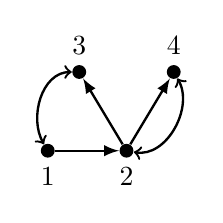
\begin{tikzpicture}
\tikzstyle{vertex}=[circle,fill=black,minimum size=5pt,inner sep=0pt]
    \node[vertex] (1) at (0,0)   [label=below:$1$]{};
    \node[vertex] (2) at (1,0) [label=below:$2$]{};
    \node[vertex] (3) at (.4,1) [label=above:$3$]{};
    \node[vertex] (4) at (1.6,1) [label=above:$4$]{};    
    \draw[->,-latex,line width=.3mm] (1) to (2);
    \draw[->,-latex,line width=.3mm] (2) to (3);
    \draw[->,-latex,line width=.3mm] (2) to (4);
    \draw[<->,thick,line width=.3mm] (1) to[out=120,in=180] (3);
    \draw[<->,thick,line width=.3mm] (2) to[out=350,in=300] (4);
  \end{tikzpicture}\qquad\qquad
  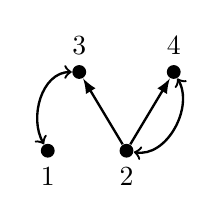
\begin{tikzpicture}
\tikzstyle{vertex}=[circle,fill=black,minimum size=5pt,inner sep=0pt]
    \node[vertex] (1) at (0,0)   [label=below:$1$]{};
    \node[vertex] (2) at (1,0) [label=below:$2$]{};
    \node[vertex] (3) at (.4,1) [label=above:$3$]{};
    \node[vertex] (4) at (1.6,1) [label=above:$4$]{};    
    \draw[->,-latex,line width=.3mm] (2) to (3);
    \draw[->,-latex,line width=.3mm] (2) to (4);
    \draw[<->,thick,line width=.3mm] (1) to[out=120,in=180] (3);
    \draw[<->,thick,line width=.3mm] (2) to[out=350,in=300] (4);
  \end{tikzpicture}
  \caption{Two simple mixed graph models. The graph on the right is obtained from the one on the lest by removing one arrow $1\to 2$.}\label{fig:ex1}
  \end{figure}

\begin{exmp}Consider the graph given on the left of Figure \ref{fig:ex1}. 
\begin{itemize}
\item give basic characteristic
\item singular locus
\item introduce the \texttt{is.equivalent.undirected} feature
\item maximum likelihood + closer analysis of the second critical point
\end{itemize}
The model is Markov equivalent to the undirected graphical model given by the following graph
\begin{center}
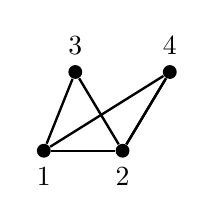
\begin{tikzpicture}
\tikzstyle{vertex}=[circle,fill=black,minimum size=5pt,inner sep=0pt]
    \node[vertex] (1) at (0,0)   [label=below:$1$]{};
    \node[vertex] (2) at (1,0) [label=below:$2$]{};
    \node[vertex] (3) at (.4,1) [label=above:$3$]{};
    \node[vertex] (4) at (1.6,1) [label=above:$4$]{};    
    \draw[-,thick,line width=.3mm] (1) to (2);
    \draw[-,thick,line width=.3mm] (2) to (3);
    \draw[-,thick,line width=.3mm] (2) to (4);
    \draw[-,thick,line width=.3mm] (1) to (3);
    \draw[-,thick,line width=.3mm] (2) to (4);
        \draw[-,thick,line width=.3mm] (1) to (4);
  \end{tikzpicture}
\end{center}
\end{exmp}



There are some other potential examples. The following graph should lead to a non-injective parametrization:
\begin{center}
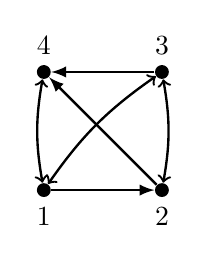
\begin{tikzpicture}
\tikzstyle{vertex}=[circle,fill=black,minimum size=5pt,inner sep=0pt]
    \node[vertex] (1) at (0,0)   [label=below:$1$]{};
    \node[vertex] (2) at (1.5,0) [label=below:$2$]{};
    \node[vertex] (3) at (1.5,1.5) [label=above:$3$]{};
    \node[vertex] (4) at (0,1.5) [label=above:$4$]{};    
    \draw[->,-latex,line width=.3mm] (1) to (2);
    \draw[->,-latex,line width=.3mm] (3) to (4);
    \draw[->,-latex,line width=.3mm] (2) to (4);
    \draw[<->,thick,line width=.3mm] (1) to[out=55,in=215] (3);
    \draw[<->,thick,line width=.3mm] (2) to[out=80,in=280] (3);
        \draw[<->,thick,line width=.3mm] (1) to[out=100,in=260] (4);
  \end{tikzpicture}
\end{center}
The following Seemingly Unrelated Regression model is equivalent to a DAG model...
\begin{center}
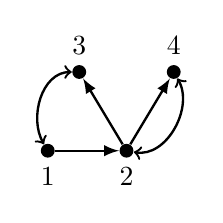
\begin{tikzpicture}
\tikzstyle{vertex}=[circle,fill=black,minimum size=5pt,inner sep=0pt]
    \node[vertex] (1) at (0,0)   [label=below:$1$]{};
    \node[vertex] (2) at (1,0) [label=below:$2$]{};
    \node[vertex] (3) at (.4,1) [label=above:$3$]{};
    \node[vertex] (4) at (1.6,1) [label=above:$4$]{};    
    \draw[->,-latex,line width=.3mm] (1) to (2);
    \draw[->,-latex,line width=.3mm] (2) to (3);
    \draw[->,-latex,line width=.3mm] (2) to (4);
    \draw[<->,thick,line width=.3mm] (1) to[out=120,in=180] (3);
    \draw[<->,thick,line width=.3mm] (2) to[out=350,in=300] (4);
  \end{tikzpicture}
\end{center}

%\section{}
%\subsection{}


\bibliographystyle{siam}
\bibliography{algebraic_statistics}
\end{document}  